
\documentclass{article}
\usepackage{CJK} 
\usepackage{graphics}
\usepackage{pgf}
\usepackage{tikz}
\usetikzlibrary{calc,shadows}
\usetikzlibrary{decorations.markings,scopes}
\usetikzlibrary{arrows,snakes,backgrounds,shapes}
\usetikzlibrary{decorations.pathmorphing}
\usepackage{listings}
\renewcommand{\ttdefault}{pcr}
\lstset{
keywordstyle=\color{blue!70},
frame=single,
basicstyle=\ttfamily\bfseries\small,
commentstyle=\small\color{red},
rulesepcolor=\color{red!20!green!20!blue!20},
tabsize=4,
numbersep=5pt,
%% backgroundcolor=\color{black!10},
showspaces=false,
showtabs=false,
extendedchars=false,
escapeinside=``,
frame=no
}

\newcommand{\blue}{\textcolor{blue}}
\newcommand{\red}{\textcolor{red}}
\newcommand{\purple}{\textcolor{purple}}


\pgfrealjobname{survey}
\begin{document}
\begin{CJK}{UTF8}{gkai} 
\beginpgfgraphicnamed{forest2btree2}

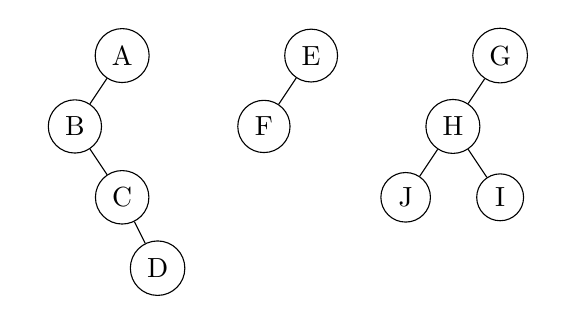
\begin{tikzpicture} [scale=0.6]
\tikzstyle{every node}=[circle,draw]
\tikzstyle{level 1}=[sibling distance=2cm]
\tikzstyle{level 2}=[sibling distance=2cm]
\tikzstyle{level 3}=[sibling distance=1.5cm]

\node at (0,0) {A} 
child {node{B} 
child [fill=none] {edge from parent[draw=none]}
child {node{C}
child [fill=none] {edge from parent[draw=none]}
child {node{D}
}
}
} 
child [fill=none] {edge from parent[draw=none]};
\node at (4,0) {E} 
child {node{F}}
child [fill=none] {edge from parent[draw=none]};
\node at (8,0) {G} 
child {node{H} child {node{J}} child {node{I}}}
child [fill=none] {edge from parent[draw=none]}
;

\end{tikzpicture}

\endpgfgraphicnamed  
\end{CJK}

\end{document}


